\documentclass{standalone}

%----------------------------------------------------------------------------------------------%
%                                 Packages and basic declarations
%----------------------------------------------------------------------------------------------%

\usepackage[utf8]{inputenc}
\usepackage{pgfplots}
\usepackage{tikz}


%----------------------------------------------------------------------------------------------%
%----------------------------------------------------------------------------------------------%
%                                            DOCUMENT STARTS
%----------------------------------------------------------------------------------------------%
%----------------------------------------------------------------------------------------------%

\begin{document}


%Tikz picture starts%

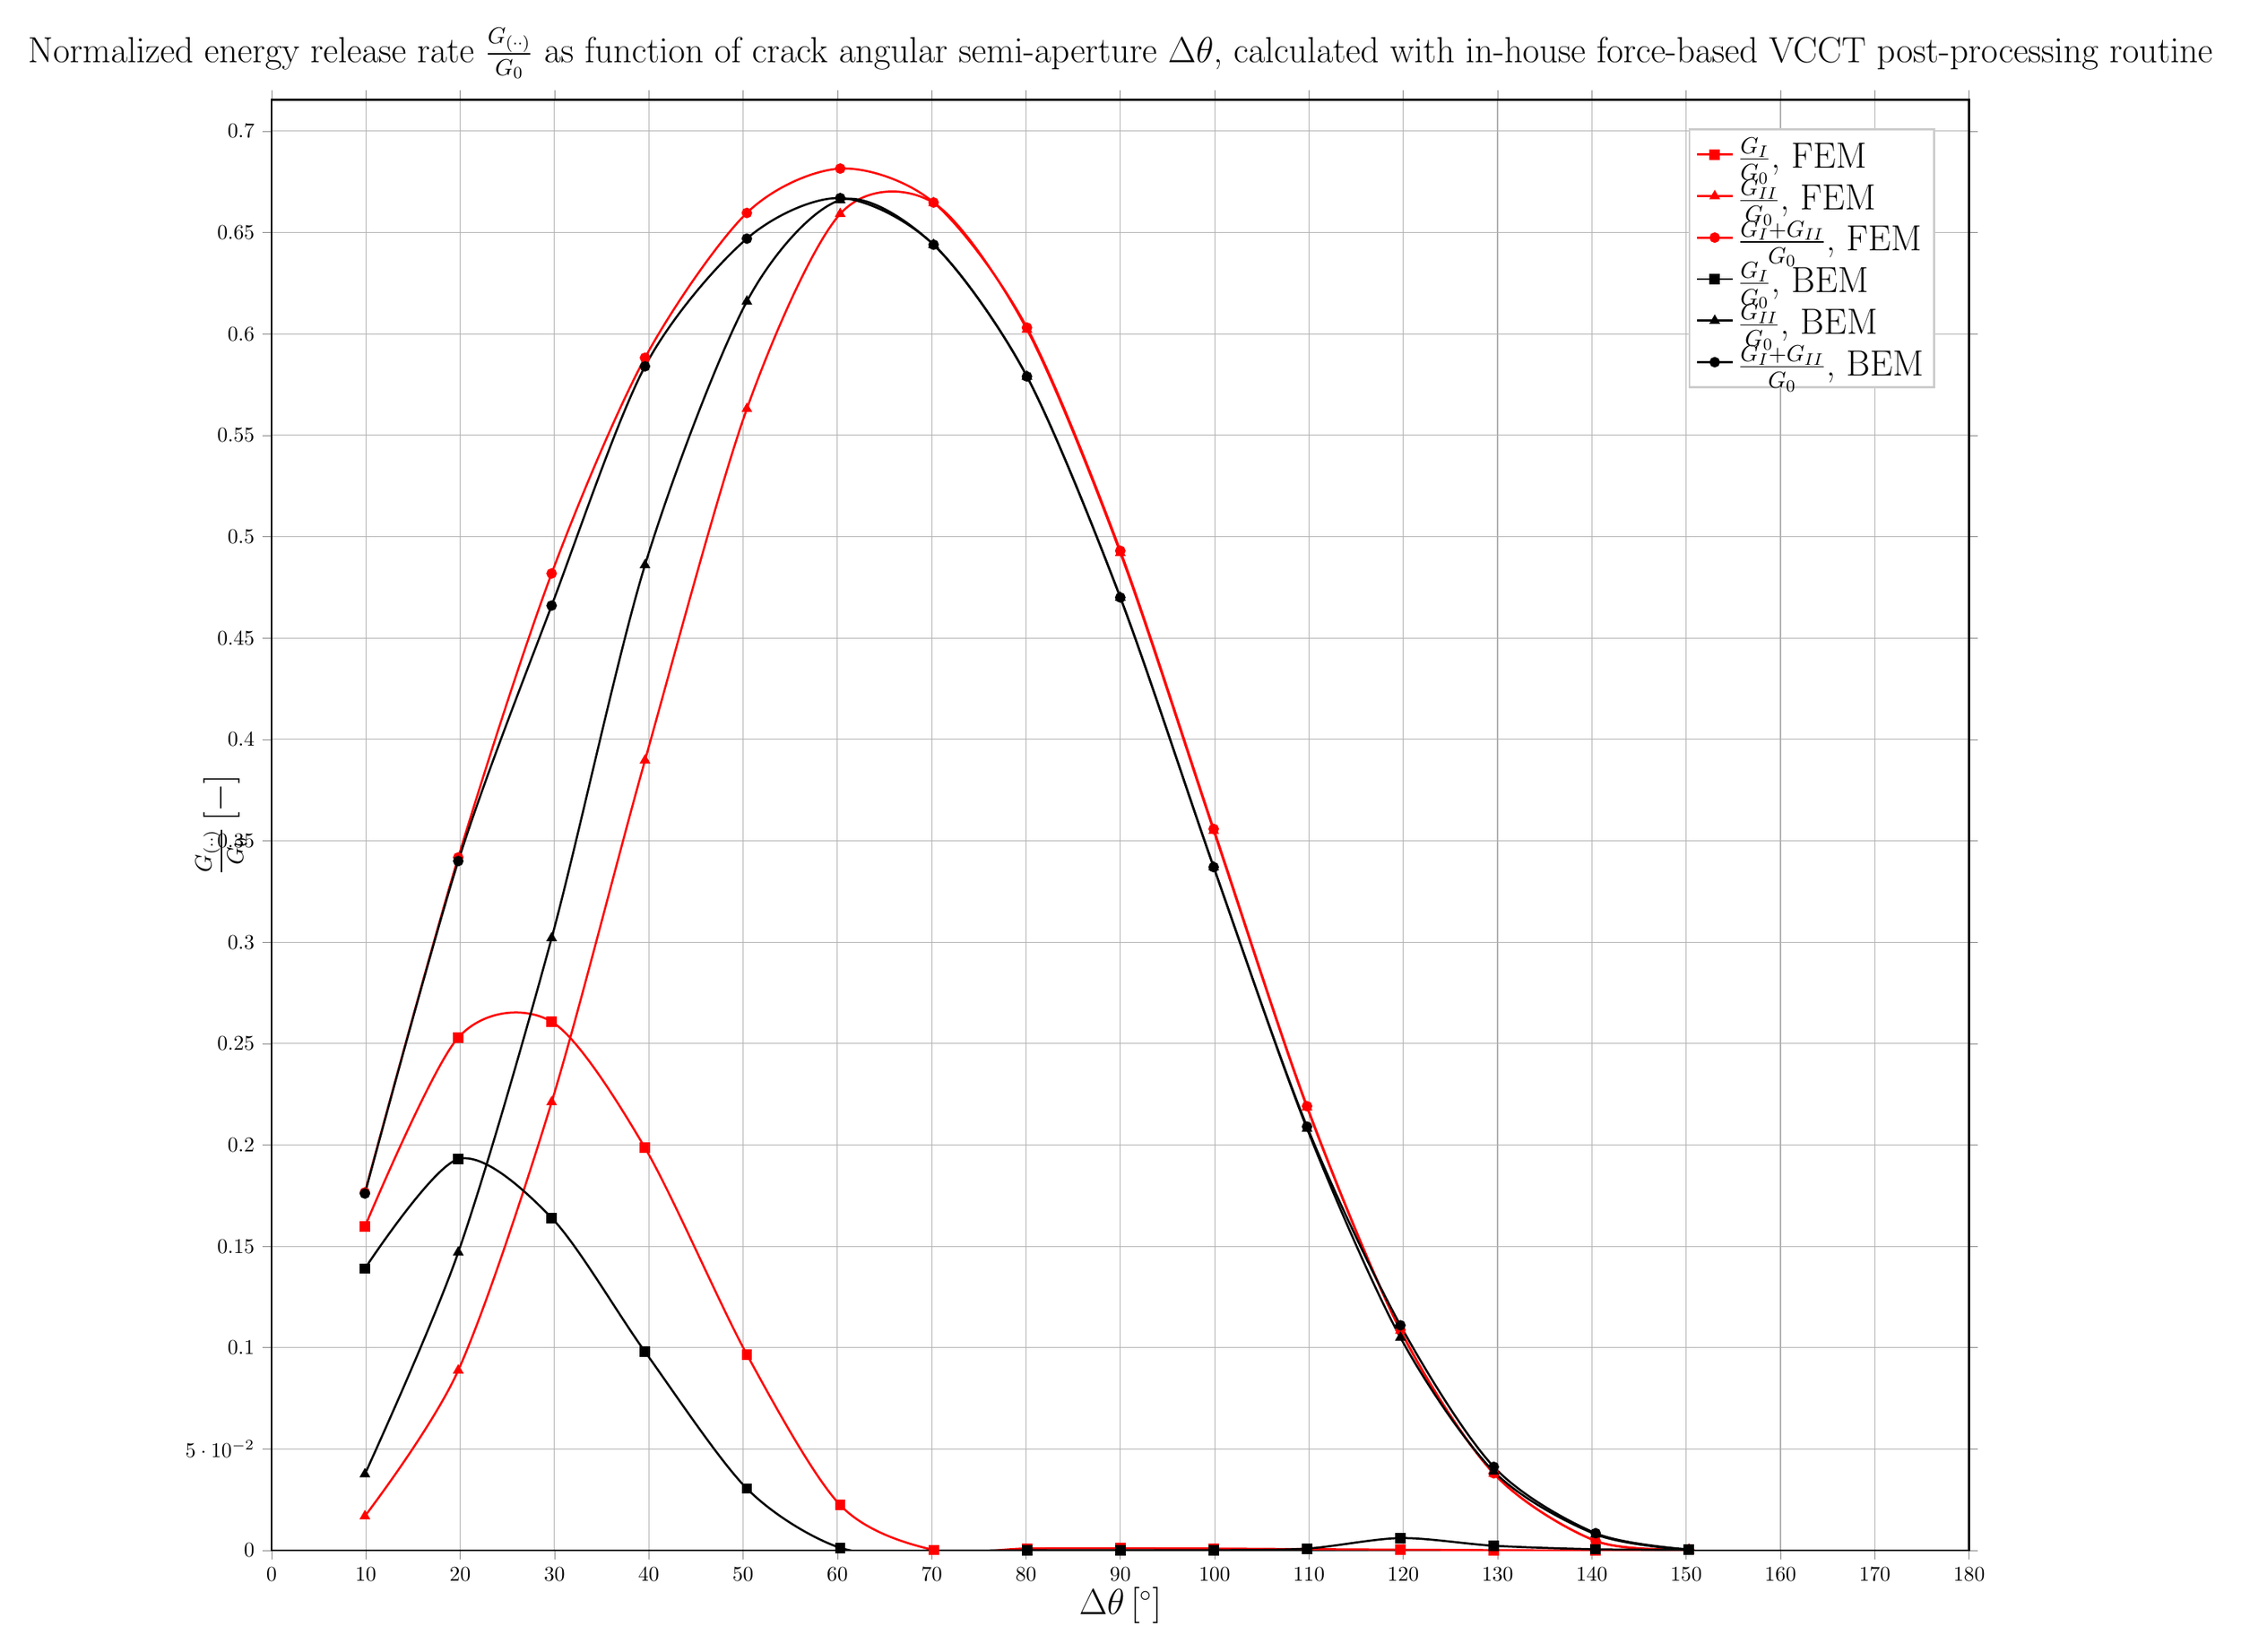
\begin{tikzpicture}

%Tikz axis starts%

\begin{axis}[width=30cm,
title={Normalized energy release rate $\frac{G_{\left(\cdot\cdot\right)}}{G_{0}}$ as function of crack angular semi-aperture  $\Delta\theta$, calculated with in-house force-based VCCT post-processing routine},
title style={font=\fontsize{16}{8}\selectfont},
xlabel style={at={(axis description cs:0.5,-0.02)},anchor=north,font=\fontsize{16}{8}\selectfont},
ylabel style={at={(axis description cs:-0.01,.5)},anchor=south,font=\fontsize{16}{8}\selectfont},
xlabel={$\Delta\theta\left[^{\circ}\right]$},ylabel={$\frac{G_{\left(\cdot\cdot\right)}}{G_{0}}\left[-\right]$},
xmin=0.0,
xmax=180.0,
ymin=0.0,
ymax=0.715635963624,
tick align=outside,
tick label style={font=\normalsize},
xtick={0.0,10.0,20.0,30.0,40.0,50.0,60.0,70.0,80.0,90.0,100.0,110.0,120.0,130.0,140.0,150.0,160.0,170.0,180.0},
xmajorgrids,
x grid style={lightgray!92.026143790849673!black},
ymajorgrids,
y grid style={lightgray!92.026143790849673!black},
line width=0.35mm,
legend style={draw=white!80.0!black,font=\fontsize{16}{12}\selectfont},
legend entries={{$\frac{G_{I}}{G_{0}}$, FEM},{$\frac{G_{II}}{G_{0}}$, FEM},{$\frac{G_{I}+G_{II}}{G_{0}}$, FEM},{$\frac{G_{I}}{G_{0}}$, BEM},{$\frac{G_{II}}{G_{0}}$, BEM},{$\frac{G_{I}+G_{II}}{G_{0}}$, BEM}},
legend cell align={left}
]

\addplot[red,smooth,mark=square*]
table{
9.90004415946 0.15967316746
19.800125885 0.252960260506
29.700111134 0.260762579173
39.5999409963 0.198539939208
50.4000580931 0.0966399501482
60.2998879554 0.0223495070457
70.1998714969 0.000202019698673
80.0999574912 0.00094106755025
90.0000025045 0.00102536895095
99.9000475177 0.000903653817829
109.800126682 0.000613764488197
119.700103393 0.000351617343608
129.599943501 0.000135666634001
140.400057182 1.72209735469e-05
150.29988363 0.000434414711528
};

\addplot[red,smooth,mark=triangle*]
table{
9.90004415946 0.0168920461338
19.800125885 0.0888136112821
29.700111134 0.221084279021
39.5999409963 0.389681926549
50.4000580931 0.563032230193
60.2998879554 0.659208553549
70.1998714969 0.664603362875
80.0999574912 0.602175206525
90.0000025045 0.491999488512
99.9000475177 0.354932862798
109.800126682 0.21847445688
119.700103393 0.108401022435
129.599943501 0.0378788852457
140.400057182 0.0046589512746
150.29988363 0.000219185208505
};

\addplot[red,smooth,mark=*]
table{
9.90004415946 0.176565213594
19.800125885 0.341773871789
29.700111134 0.481846858194
39.5999409963 0.588221865757
50.4000580931 0.659672180341
60.2998879554 0.681558060594
70.1998714969 0.664805382573
80.0999574912 0.603116274076
90.0000025045 0.493024857463
99.9000475177 0.355836516616
109.800126682 0.219088221368
119.700103393 0.108752639778
129.599943501 0.0380145518797
140.400057182 0.00467617224815
150.29988363 0.000653599920033
};

\addplot[black,smooth,mark=square*]
table{
9.90004415946 0.139
19.800125885 0.193
29.700111134 0.164
39.5999409963 0.098
50.4000580931 0.0305
60.2998879554 0.00127
70.1998714969 -4.79e-05
80.0999574912 6.85e-05
90.0000025045 0.000112
99.9000475177 0.000112
109.800126682 0.000895
119.700103393 0.00607
129.599943501 0.00229
140.400057182 0.000552
150.29988363 0.000306
};

\addplot[black,smooth,mark=triangle*]
table{
9.90004415946 0.0376
19.800125885 0.147
29.700111134 0.302
39.5999409963 0.486
50.4000580931 0.616
60.2998879554 0.666
70.1998714969 0.644
80.0999574912 0.579
90.0000025045 0.47
99.9000475177 0.337
109.800126682 0.208
119.700103393 0.105
129.599943501 0.0389
140.400057182 0.00792
150.29988363 0.000165
};

\addplot[black,smooth,mark=*]
table{
9.90004415946 0.176
19.800125885 0.34
29.700111134 0.466
39.5999409963 0.584
50.4000580931 0.647
60.2998879554 0.667
70.1998714969 0.644
80.0999574912 0.579
90.0000025045 0.47
99.9000475177 0.337
109.800126682 0.209
119.700103393 0.111
129.599943501 0.0412
140.400057182 0.00847
150.29988363 0.000471
};

\end{axis}
%Tikz axis ends%


\end{tikzpicture}
%Tikz picture ends%


\end{document}

%----------------------------------------------------------------------------------------------%
%----------------------------------------------------------------------------------------------%
%                                            DOCUMENT ENDS
%----------------------------------------------------------------------------------------------%
%----------------------------------------------------------------------------------------------%

